\documentclass[acmsmall,anonymous,review]{acmart}

\AtBeginDocument{%
  \providecommand\BibTeX{{Bib\TeX}}}
\setcopyright{none}
\settopmatter{printacmref=false,printccs=true,printfolios=true}
\renewcommand\footnotetextcopyrightpermission[1]{}
\acmJournal{JDIQ}
\acmYear{2026}
\acmDOI{}
\hypersetup{
  pdfauthor={Anonymous Author(s)},
  pdftitle={Experience: Auditing LLM-Assisted Evidence Synthesis Without Ground Truth}
}

\usepackage{booktabs}
\usepackage{tabularx}
\usepackage{array}
\usepackage{graphicx}
\usepackage{xcolor}
\usepackage{microtype}
\microtypesetup{expansion=false}
\usepackage{enumitem}
\graphicspath{{figures/}}

\newcolumntype{Y}{>{\raggedright\arraybackslash}X}
\newcommand{\NA}{\textsc{n/a}}

\title{Experience: Auditing LLM-Assisted Evidence Synthesis Without Ground Truth}

\author{Anonymous Author(s)}
\affiliation{%
  \institution{Anonymous Institution}
  \country{Anonymous}}
\email{anonymous@example.invalid}

\begin{abstract}
Large language models are increasingly used to create and evaluate structured data, but archived workflows often lack an external reference standard. We report an experience-based data-quality audit of an LLM-assisted evidence-synthesis workflow spanning 20 purposively selected cases. The archive contains 95,292 retrieved records, 94,522 post-deduplication records, 19,276 records labelled INCLUDE, 11,500 extracted records, and 90,554 requested field values. The present research question was adopted after inspection of the archived outputs and a later repeatability experiment; it was not preregistered. We therefore do not estimate screening accuracy, extraction accuracy, or evaluator validity. Instead, we quantify three properties that remain identifiable. First, excluding 36,881 UNVERIFIABLE fields changes the evaluator-labelled CORRECT share from 58.39\% to 98.52\%, solely by changing the denominator. Second, in a separate three-call experiment on 500 frozen extraction items, the design-weighted probability of changing null status was 1.92\% (case-cluster bootstrap 95\% interval 0.60\%--4.34\%); among 154 all-non-null categorical items, deterministic normalization changed exact agreement from 21.58\% to 46.13\%. Third, ten extraction schemas yielded 927 complete estimate-and-interval rows, yet none recorded both study-level linkage and variance information needed to establish synthesis readiness. Model identity and historical failure incidence were not recoverable because provenance and call-status records were absent. The experience shows how denominator policy, output representation, and downstream schema design can materially change quality claims even when factual accuracy cannot be measured.
\end{abstract}

\ccsdesc[500]{Information systems~Data provenance}
\ccsdesc[500]{Information systems~Data extraction and integration}
\ccsdesc[300]{General and reference~Empirical studies}

\keywords{data quality, large language models, evidence synthesis, provenance, repeatability, missing data, data contracts}

\begin{document}
\maketitle

\section{Introduction}

LLM-assisted workflows increasingly turn unstructured text into decisions and structured records. Evidence synthesis is a useful testbed because it connects several data-intensive stages: bibliographic retrieval, deduplication, record screening, field extraction, output evaluation, and statistical aggregation. Errors or missing information at one stage constrain what can be claimed at later stages. Reporting a high agreement percentage at the extraction stage, for example, says little unless its denominator and abstention policy are explicit. A populated effect-size column does not establish that the rows form a valid meta-analysis dataset.

External reference data are the usual basis for accuracy claims. In evidence synthesis, a defensible reference would require independent human screening, source-level extraction, and adjudication. Such a reference was not available for the archived workflow examined here. The absence of ground truth does not make every data-quality question unanswerable. It changes the question. Completeness, provenance, operational observability, repeatability, denominator sensitivity, and fitness for an intended downstream analysis can be audited directly, whereas factual accuracy and evaluator validity cannot.

This paper reports an experience-based audit of a 20-case LLM-assisted evidence-synthesis workflow. The cases span health and clinical research, social and behavioral science, education, environmental research, and computer science. A prior report used the same archive to study validation and error propagation \cite{anonymous2026prior}. The present audit re-examines which of those quantities the retained evidence can support. It found that the historical screening model alias was inconsistent across retained artifacts; terminal failures had been mapped to ordinary analytical states without an event log; and the extraction schemas did not retain the study-level and uncertainty information needed for a defensible meta-analysis. We therefore amended the research question after observing the archived and prospective results. This post-outcome change is disclosed throughout the paper and in an append-only protocol amendment.

The contribution is deliberately bounded. Provenance capture, operational logging, data contracts, fitness for use, abstention-aware evaluation, and representation-sensitive agreement are established ideas \cite{w3cprov2013,polyzotis2021mlmd,sre2016monitoring,wang1996beyond,shacl2017,wen2025abstention}. We do not propose a new standard for any of them. We quantify what their absence or underspecification did to this archive. The analysis makes three primary contributions:

\begin{enumerate}[leftmargin=*,itemsep=2pt]
  \item It measures a 40.12 percentage-point change in the displayed evaluator agreement when UNVERIFIABLE fields are removed from the denominator.
  \item It separates null-state stability from non-null representation in a three-call experiment, showing largely stable null status but a 24.55-point normalization effect for categorical exact agreement.
  \item It demonstrates that 927 complete estimate-and-interval rows still do not establish synthesis readiness when schemas omit study linkage, effect-measure metadata, variance, time point, and dependence identifiers.
\end{enumerate}

Two additional findings define the limits of the evidence. The historical screening model cannot be attributed to a specific alias because the manuscript, repository documentation, and committed script disagree. Historical call failures cannot be counted because no call-status ledger was retained and terminal failures shared values with legitimate outputs. These are identifiability findings, not performance estimates.

\section{Related Work and Novelty Boundary}

\subsection{Data quality is broader than accuracy}

Data quality has long been treated as multidimensional and dependent on use \cite{wang1996beyond}. Completeness, consistency, accessibility, interpretability, and fitness for a particular task can matter even when factual accuracy is unknown. Study-specific data-quality assessment similarly distinguishes generic conformance from fitness for a concrete analysis \cite{preserve2024}. Declarative constraint systems such as SHACL formalize types, cardinalities, and cross-field requirements \cite{shacl2017}. Our schema audit applies this downstream-oriented view: the relevant question is not merely whether numeric fields are populated, but whether the data model records the estimand, uncertainty, unit of independence, and dependence structure required by a synthesis.

\subsection{Provenance and operational observability}

W3C PROV represents linked entities, activities, agents, and derivations \cite{w3cprov2013}; scientific-workflow provenance distinguishes a planned workflow from the execution that actually produced an artifact \cite{davidson2008provenance}. Machine-learning metadata systems make runs, inputs, outputs, and contexts explicit \cite{polyzotis2021mlmd}. Operational guidance likewise treats requests, outcomes, errors, latency, and retries as first-class events \cite{sre2016monitoring,otel2025genai}. The present archive illustrates a specific consequence of violating these principles: executable code alone cannot establish the identity or reliability of an earlier execution when outputs predate the committed implementation and no per-call trace exists.

\subsection{LLM evaluation and evidence synthesis}

Research on LLM evaluation distinguishes lexical identity from semantic equivalence and documents limitations of LLM-as-judge designs \cite{kamalloo2023qa,zheng2023judge}. Abstention also changes the target estimand: conditional performance among answered items is not performance across all attempted items \cite{wen2025abstention}. Repeated calls can vary under nominally deterministic settings \cite{pagnamenta2025nondeterminism}. We decompose exact agreement, deterministic normalization, token-set equality, and null-state transitions on the same frozen inputs.

Evidence-synthesis guidance emphasizes human accountability \cite{flemyng2025ai}, while a recent systematic review documents both the potential and limitations of generative AI \cite{clark2025genai}. Because this archive has no independent reference labels, we examine the measurement and infrastructure conditions required before a benchmark claim would be meaningful.

\section{Workflow Archive and Audit Design}

\subsection{Twenty-case archive}

The archive contains 20 purposively selected cases distributed across five domains. Cases vary in corpus size, terminology, prevalence of historical INCLUDE labels, retrieval source, and extraction schema. They are design cases rather than a probability sample of disciplines; no population-level domain comparison is attempted. Across cases, the historical summaries report 95,292 records before within-case deduplication and 94,522 retained records. Screening assigned 19,276 INCLUDE labels. Extraction produced 11,500 record rows and requested 90,554 field values.

Six cases reached or exceeded configured retrieval limits; the supplement's retrieval-limit table lists each case, source, limit, and retained count. Historical source-reported totals and removed duplicate pairs were not saved, so corpus completeness and false merges cannot be reconstructed. Metadata completeness among retained records was 99.99\% for title, 98.95\% for abstract, 86.07\% for DOI, and 98.99\% for year. Language and source-native identifiers were not collected and are therefore unmeasured rather than zero.

The historical screening outputs contain a three-way provenance conflict. The committed script declares \texttt{gpt-4.1-mini}; the empirical README names \texttt{gpt-4o-mini}; and the prior report names \texttt{gpt-4o}. The 94,522 screened rows retain no requested model, returned model, request identifier, timestamp, prompt hash, or system fingerprint. The files predate the first reachable commit of the screening script. We therefore record the generating screening alias as unresolved. Historical extraction and evaluator materials consistently declare \texttt{gpt-4o-mini}, but the calls likewise lack returned model identifiers and version fingerprints.

\subsection{Post-outcome amendment and estimands}

An initial protocol proposed human-referenced screening and extraction validation, evaluator error injection, meta-analysis, and calibrated propagation. After inspection of the archive and the later repeatability results, those branches were removed from the current paper because no external reference standard was available. The revised question asks which data-quality properties remain observable and identifiable without external truth labels, and how denominator rules, output representation, provenance gaps, failure-state encoding, and schema design affect those properties. The amendment was made after outcome inspection and was not preregistered. The amendments are summarized in the supplement and supplied verbatim in the anonymous artifact.

The audit separates three measurable effects from two identifiability diagnoses. The measurable effects are: (1) the change in evaluator-labelled CORRECT share under two declared denominators; (2) the probability of a null-state change and representation-sensitive agreement in a separate repeated-call experiment; and (3) the coverage of schema fields required for downstream synthesis. The identifiability diagnoses concern historical model identity and operational failure incidence. Accuracy, semantic equivalence, evaluator sensitivity or specificity, and pooled effects are outside scope.

\subsection{Evaluator denominator analysis}

The historical evaluator assigns CORRECT, INCORRECT, or UNVERIFIABLE to each requested field. We compute the CORRECT share first over all requested fields and then over only fields assigned CORRECT or INCORRECT. The numerator is identical. The contrast therefore isolates the effect of denominator policy. We report the complete label distribution so that abstention is not hidden.

\subsection{Prospective same-request repeatability}

A separate prospective experiment sampled 200 screening records and 500 extraction fields from frozen historical inputs. Each item was submitted three times to the \texttt{gpt-5-mini} alias. The experiment produced 600 successful screening calls and 1,500 successful extraction calls. It used prompts and strict response schemas that differed from the historical workflow and does not estimate historical-model repeatability. The client requested \texttt{temperature=0}; the saved responses expose neither the effective server-side decoding configuration nor a system fingerprint. We therefore describe observed same-request repeatability rather than deterministic decoding.

The screening frame first selected up to 30 records within each case-by-historical-label stratum by a seeded SHA-256 rank. The experiment then ranked those 1,192 frame records by a second seeded SHA-256 hash of the sample identifier and selected the first 200, independent of file order. The resulting subset covered all 20 cases and contained 96 historical INCLUDE and 104 historical EXCLUDE records. Because the second stage was deterministic rather than a probability sample, we report the realized stability proportion and complete transition counts without a population claim.

For extraction, items were sampled within case and field strata with recorded selection probabilities. We use inverse-probability weights, $w_i=1/\pi_i$, where $\pi_i$ is item $i$'s sampling probability. Uncertainty intervals come from 10,000 bootstrap resamples of the 20 case clusters with a fixed random seed.

Each extraction item is classified as all-null, all-non-null, or mixed-null across its three calls. For all-non-null values we compare four representations: raw parsed equality; deterministic normalization; token-set equality; and a lexical-similarity threshold. Normalization applies Unicode NFKC, case folding, separator and punctuation normalization, whitespace normalization, and a small declared British-to-American spelling map. Token-set equality additionally ignores order and repeated tokens. Lexical similarity is the minimum pairwise SequenceMatcher ratio across the three normalized outputs; thresholds are sensitivity analyses, not validated semantic-equivalence rules.

\subsection{Downstream schema audit}

Each case-specific extraction schema was checked for fields needed to determine whether its rows could support an inverse-variance meta-analysis. Requirements included a study-level linkage identifier, outcome construct, analysis time point, effect-measure label or effect-specific estimate, interval or variance, and a dependence identifier. We counted complete numeric estimate-and-interval rows separately from schema coverage. This distinction tests whether row-level numeric completeness can be mistaken for analysis readiness.

\section{Results}

\subsection{Three measured consequences}

Table~\ref{tab:consequences} gives the empirical center of the paper. The first two effects arise from measurement policy rather than changes to underlying model outputs. The third shows that populated numeric values do not compensate for missing analytical context.

\begin{table*}[t]
\caption{Measured consequences and the claims they support. Accuracy, semantic validity, and historical failure incidence are outside the identified quantities.}
\label{tab:consequences}
\small
\begin{tabularx}{\textwidth}{p{0.19\textwidth}Y Y Y}
\toprule
\textbf{Control} & \textbf{Observed consequence} & \textbf{Supported interpretation} & \textbf{Not identified} \\
\midrule
Denominator-explicit reporting & CORRECT is 52,877/90,554 (58.39\%) over all requested fields and 52,877/53,673 (98.52\%) after excluding 36,881 UNVERIFIABLE fields; a 40.12-point increase. & The displayed percentage is highly sensitive to the declared denominator. & Extraction accuracy or evaluator validity. \\
\addlinespace
Representation- and null-aware repeatability & Weighted mixed-null probability is 1.92\% (0.60\%--4.34\%). For 154 all-non-null categorical items, raw exact is 21.58\% and normalized exact is 46.13\%; a 24.55-point increase. & Null states were largely but not perfectly stable; categorical agreement depends materially on representation. & Semantic equivalence or factual correctness. \\
\addlinespace
Downstream-first schema design & Ten schemas yield 927 complete estimate-and-interval rows; each of four required fields is individually absent from all 20 schemas: study linkage, effect-measure metadata, variance/standard error, and dependence. & Numeric completeness does not establish synthesis readiness. & A valid pooled effect or calibrated propagation result. \\
\bottomrule
\end{tabularx}
\end{table*}

\subsection{Denominator restriction changes the reported evaluator percentage}

The 90,554 requested fields received 52,877 CORRECT labels, 796 INCORRECT labels, and 36,881 UNVERIFIABLE labels. Using all requested fields, the CORRECT share is 58.39\%. Restricting the denominator to the 53,673 fields labelled CORRECT or INCORRECT produces 98.52\%. No evaluator decision changes between these calculations; the 40.12-point increase is entirely a denominator effect.

Null values explain much of the UNVERIFIABLE category. Among 36,641 null extraction cells, 36,423 were UNVERIFIABLE. This near-equivalence is expected because a null supplies no candidate value to verify. The informative exceptions are 198 null fields labelled CORRECT, 20 null fields labelled INCORRECT, and 458 non-null fields labelled UNVERIFIABLE. These discordant cells reveal inconsistent treatment or source insufficiency, but they do not supply a truth label.

Figure~\ref{fig:denominators} combines the record-level stage ledger with the two field-level evaluator denominators. It also shows an extraction-coverage limitation: Cases 16--20 contain 8,776 INCLUDE labels but only 1,000 archived extraction rows. The 7,776 omitted records are 88.61\% of INCLUDE labels in those five cases and 40.34\% of all 19,276 INCLUDE labels across the archive.

\begin{figure*}[t]
  \centering
  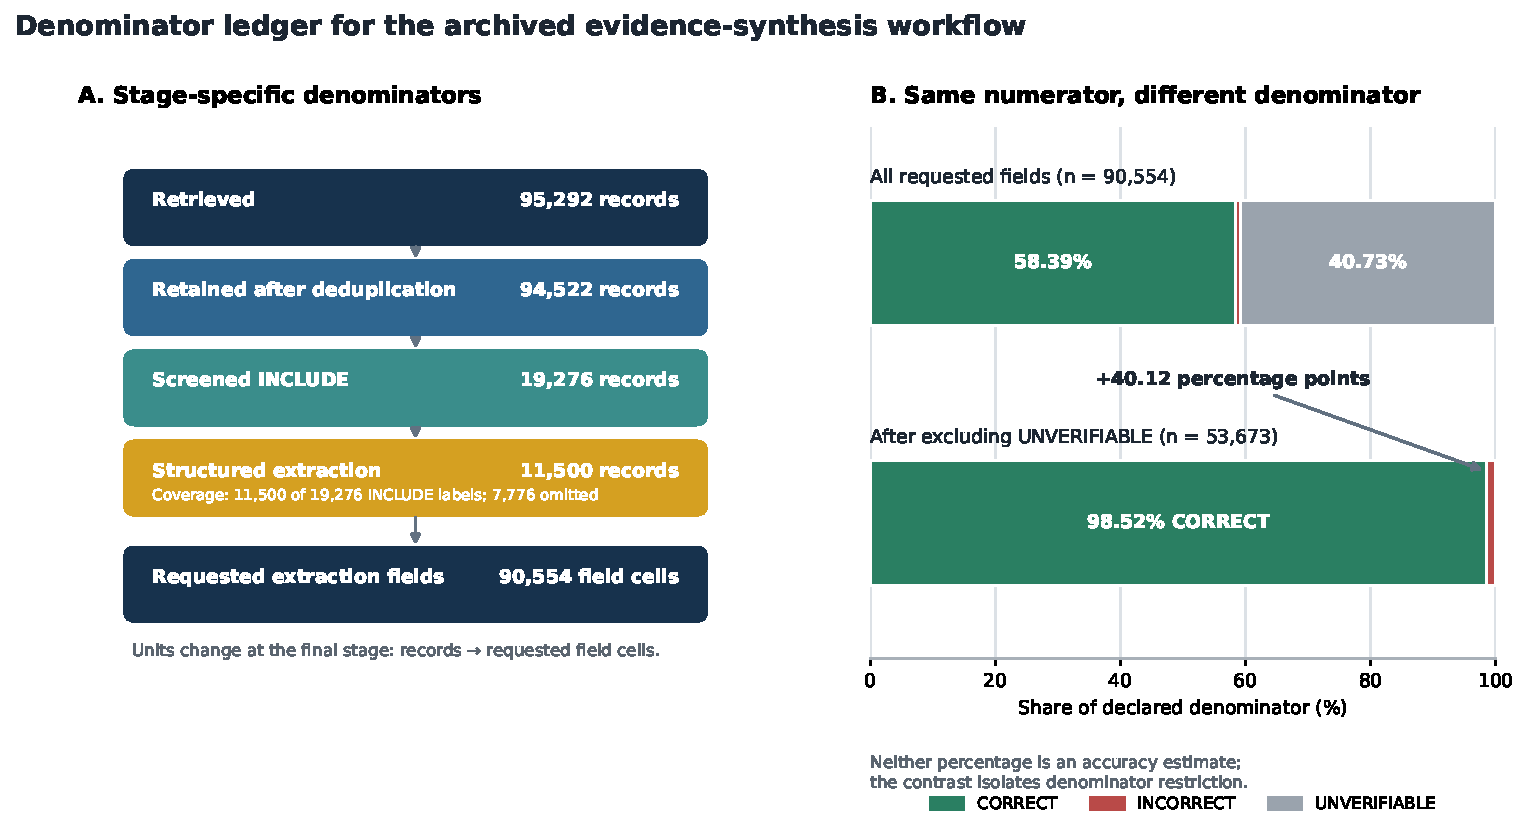
\includegraphics[width=\textwidth]{denominator_ledger.pdf}
  \Description{A two-panel denominator ledger. The left panel shows 95,292 retrieved records, 94,522 retained records, 19,276 INCLUDE decisions, 11,500 extracted records, and 90,554 requested field cells. The right panel shows the same 52,877 CORRECT labels as 58.39 percent of all requested fields and 98.52 percent after excluding UNVERIFIABLE fields.}
  \caption{Stage-specific units and denominators. Record counts should not be mixed with requested field-cell counts. The right panel shows the same CORRECT numerator under the full requested-field denominator and the restricted evaluator-decidable denominator.}
  \label{fig:denominators}
\end{figure*}

\subsection{Screening labels and null states are largely stable, while categorical agreement is representation-sensitive}

Among the 200 screening records, 190 retained the same label across all three calls (95.00\%). Of 400 adjacent repeat comparisons, 13 changed label: seven INCLUDE-to-EXCLUDE and six EXCLUDE-to-INCLUDE. This is prospective same-request stability, not screening accuracy or historical-model repeatability.

The design-weighted probability that an extraction item changed null status at least once across three calls was 1.92\%, with a case-cluster bootstrap 95\% interval of 0.60\%--4.34\%. In the realized stratified sample, 36 of 500 items (7.20\%) were mixed-null. These are different estimands: the first represents the target induced by the sampling weights; the second describes the selected sample. The remaining sample contained 160 all-null items and 304 all-non-null items. The 36 mixed-null items comprised 23 categorical and 13 numeric fields and generated 44 adjacent null-state transitions. Null states were therefore largely, but not perfectly, stable.

Table~\ref{tab:repeatability} reports all-non-null agreement. For categorical fields, deterministic normalization changes the weighted exact estimate from 21.58\% to 46.13\%. Token-set equality yields 47.79\%, while 53.35\% meet the minimum pairwise lexical-similarity threshold of 0.80. The case-cluster bootstrap interval for normalized categorical exact agreement is 34.76\%--56.34\%. Numeric fields are more stable, but their normalized exact estimate of 88.55\% (81.18\%--95.96\%) still leaves 11.45\% design-weighted non-agreement. The residual variation may include both harmless formatting differences and substantive changes; without a semantic reference, those components cannot be separated.

\begin{table}[t]
\caption{Design-weighted agreement for all-non-null extraction items in the separate three-call \texttt{gpt-5-mini} experiment.}
\label{tab:repeatability}
\small
\begin{tabular}{lrrrrr}
\toprule
\textbf{Type} & \textbf{$n$} & \textbf{Raw} & \textbf{Normalized} & \textbf{Token set} & \textbf{Lexical $\geq .80$} \\
\midrule
Categorical & 154 & 21.58\% & 46.13\% & 47.79\% & 53.35\% \\
Numeric & 150 & 88.40\% & 88.55\% & 88.55\% & 90.22\% \\
\bottomrule
\end{tabular}
\end{table}

\subsection{Complete numeric rows do not establish synthesis readiness}

Ten of the 20 schemas include estimate and confidence-interval fields. Across them, 927 rows have complete numeric estimates and interval bounds, and seven cases pass a naive threshold of five such rows. Nevertheless, none of the 20 schemas includes a study-level linkage identifier, a dedicated effect-measure metadata field, a variance or standard-error field, or a dependence identifier. Report DOIs are retained when available, but a DOI identifies a report rather than grouping multiple reports from the same underlying study. Only one schema names an effect-specific estimate field (\texttt{hazard\_ratio}); the other nine use a generic \texttt{effect\_size}. Only two schemas include an analysis time point.

The schema coverage result is therefore 0/20 for the joint presence of study linkage, effect-measure metadata, variance or standard error, and a dependence identifier. This result does not show that the extracted numbers are false. It shows that the data model did not record enough information to establish a common estimand, independent-study set, and uncertainty structure. Statistical pooling was consequently not attempted.

\subsection{Provenance and failure incidence are not reconstructable}

The three conflicting screening aliases prevent model-specific attribution of all 94,522 historical screening labels. Treating the committed script as definitive would be unjustified because the outputs predate the first reachable script commit. The extraction and evaluator alias is consistently declared but not verified per call. These gaps illustrate the difference between code provenance and execution provenance.

Historical terminal failures are similarly non-identifiable. The screening code returned EXCLUDE after terminal failure, the extraction code returned all-null fields, and the evaluator returned all-UNVERIFIABLE labels. Each fallback collides with a valid analytical state. No event table records attempts, retries, status codes, parse outcomes, or errors. Counting all EXCLUDE, all-null, or all-UNVERIFIABLE observations as failures would therefore be a trivial worst case rather than an empirical rate.

A reviewer might reasonably ask why the workflow was not rerun with logging. A new logged run could estimate the operational failure rate of a current implementation. It could not recover the historical rate because the requested and returned models, provider infrastructure, prompt and schema contracts, client code, retry behavior, rate limits, corpus state, and execution period would differ. The historical execution is the estimand of this audit. Substituting a later run would answer a separate prospective question and create false retrospective precision.

\section{Experience-Based Design Lessons}

\subsection{Maintain a denominator ledger across changing units}

The workflow moves from bibliographic records to screening decisions, extracted records, requested field cells, non-null values, and evaluator-decidable cells. A single percentage cannot travel across these units without an explicit denominator policy. Every reported quality statistic should name its unit, numerator, denominator, excluded states, and reason for exclusion. Abstention or unverifiability should be reported jointly with conditional agreement rather than removed silently.

\subsection{Separate operational state from analytical value}

A technical failure is not a negative screening decision, a source-unreported value, or an evaluator abstention. A production event record should be written for every attempt and should include a logical request identifier, attempt number, requested and returned model identifiers, prompt and schema hashes, timestamps, latency, status, response or error category, and retry disposition. Analytical values should be emitted only after the operational record establishes successful completion and parsing. This recommendation implements established observability practice rather than introducing a new logging standard \cite{sre2016monitoring,otel2025genai}.

\subsection{Treat output representation as part of the metric}

Raw exact agreement is reproducible and strict, but it is not representation-neutral. Normalization approximately doubled categorical exact agreement in this experiment, while barely changing numeric agreement. A report should therefore separate null-state transitions, raw equality, declared normalization, token-based comparisons, and any semantic assessment. Normalization rules must be versioned because changing them changes the estimand. Semantic correctness still requires an external reference or a validated adjudication process.

Where a categorical target has a finite domain, the extraction contract should use a versioned controlled vocabulary with explicit OTHER and UNKNOWN states. This turns out-of-vocabulary responses into observable contract violations instead of allowing surface variation to be counted indiscriminately as instability.

\subsection{Record execution provenance, not only configuration prose}

A manuscript statement, README, and script can each be internally plausible while disagreeing about what executed. The durable unit should be a run record that links the exact input snapshot, prompt, response schema, parser, client code, requested model, returned model, provider fingerprint when available, and generated outputs. The record must be written at execution time and should not rely on later reconstruction from repository state \cite{w3cprov2013,davidson2008provenance,polyzotis2021mlmd}.

\subsection{Design schemas backward from the intended analysis}

Strict JSON conformance is not equivalent to scientific adequacy. If meta-analysis is a possible downstream use, the extraction contract should encode the study identifier, report identifier, outcome construct, effect measure and scale, time point, comparison, estimate, uncertainty, sample size where relevant, and dependence grouping. These fields should be linked by cross-field rules. The schema should fail early when the planned estimand cannot be represented, rather than allowing hundreds of apparently complete rows that cannot be combined.

\section{Limitations}

This study has five principal limitations. First, the research question is post-outcome. It was adopted after inspection of the archived outputs and prospective repeatability results, so the numerical findings are descriptive and require independent replication. Second, the 20 cases were purposively selected and do not support population claims about disciplines, retrieval systems, or LLM-assisted evidence synthesis generally. Third, there is no independent human or source-level reference. The study cannot estimate screening accuracy, extraction accuracy, evaluator validity, semantic equivalence, or factual correctness.

Fourth, the repeatability experiment concerns a later \texttt{gpt-5-mini} execution with different prompts and schemas. It does not characterize the unresolved historical screening system or the historically declared extraction and evaluation alias. The client requested \texttt{temperature=0}, but effective server-side decoding parameters were not exposed. Fifth, historical retrieval totals, removed duplicate pairs, and event logs were not retained. Corpus completeness, false-merge rates, and operational failure incidence remain unidentifiable.

The audit also excludes a pooled meta-analysis and calibrated error-propagation simulation. This is a methodological restriction rather than a missing result. The archived schemas do not establish a common estimand or independent-study set, and no external error model is available. Producing pooled estimates under those conditions would add numerical precision without evidential validity.

\section{Conclusion}

An LLM-assisted workflow can produce a large structured archive while leaving its most attractive quality claims unidentified. In this experience, the measurable consequences were not hidden model accuracies. They were changes induced by denominator policy, output representation, and schema design. Removing UNVERIFIABLE fields raised a displayed CORRECT share from 58.39\% to 98.52\%. Deterministic normalization raised all-non-null categorical exact agreement from 21.58\% to 46.13\%. Nine hundred twenty-seven complete estimate-and-interval rows still lacked the linkage and uncertainty fields needed to establish synthesis readiness. Meanwhile, missing execution records made historical model identity and failure incidence unrecoverable.

These results support a practical rule: data-quality controls must be designed around downstream claims. Denominator ledgers, event records, provenance, appropriate agreement measures, and analysis-driven schemas do not replace accuracy validation. They determine whether accuracy, reliability, and synthesis can be measured at all.

\section*{Data and Code Availability}

A double-anonymous review artifact is supplied as online supplementary material. It contains the case-by-field-type-by-null-status-by-verdict count cube, screening and extraction repeatability summaries, schema tables, figure-generation code, dependency specification, checksums, and automated tests needed to reproduce the reported results. It excludes raw bibliographic text, old manuscripts, Git history, author-identifying metadata, and the preserved historical repository snapshot.

\bibliographystyle{ACM-Reference-Format}
\bibliography{references}

\end{document}
